%%%%%%%%%%%%%%%%%%%%%%%%%%%%%%%%%%%%%%%%%%%%%%%%%%%%%%%%%%%%%%%%%%%%%%%%%%%%%%%
%% StuPro B, "Programmierumgebung Offener Antrieb" (POA)
%% Handbuch
%% $Id: handbuch.tex,v 1.14 2004/03/05 12:19:38 neco Exp $
%%%%%%%%%%%%%%%%%%%%%%%%%%%%%%%%%%%%%%%%%%%%%%%%%%%%%%%%%%%%%%%%%%%%%%%%%%%%%%%
\documentclass[a4paper,titlepage,12pt,ngerman]{scrbook}
\usepackage{../common/header}

\RCSdef $Revision: 1.14 $
\RCSdef $Date: 2004/03/05 12:19:38 $

\newcommand\version{Version 1.0 \xspace}

\begin{document}

%%%%%%%%%%%%%%%%%%%%%%%%%%%%%%%%%%%%%%%%%%%%%%%%%%%%%%%%%%%%%%%%%%%%%%%%%%%%%%%
%% Deckblatt

\begin{titlepage}
\renewcommand{\thefootnote}{\fnsymbol{footnote}}
{\Huge
\raggedright
\textbf{POA} \\
\huge Programmierumgebung offener Antrieb
\rule{\textwidth}{0.75pt}
\par
}
\begin{flushleft}
\normalsize
\version
\vfill

\begin{figure}[htbp]
\begin{center}

\includegraphics[width=15cm]{poa-logo}
\end{center}
\end{figure}

\end{flushleft}
\vfill

{\parindent=0cm
\Huge Handbuch
\normalsize
\par zum Release 0.3.0
\par 
Screenshots in diesem Dokument wurden unter Linux gemacht.\newline
Es k"onnte unter Umst"anden unter Windows Abweichungen geben.
}


\setcounter{footnote}{0}
\end{titlepage}


%%%%%%%%%%%%%%%%%%%%%%%%%%%%%%%%%%%%%%%%%%%%%%%%%%%%%%%%%%%%%%%%%%%%%%%%%%%%%%%
%% Inhaltsverzeichnis

\tableofcontents

%%%%%%%%%%%%%%%%%%%%%%%%%%%%%%%%%%%%%%%%%%%%%%%%%%%%%%%%%%%%%%%%%%%%%%%%%%%%%%%
%%%%%%%%%%%%%%%%%%%%%%%%%%%%%%%%%%%%%%%%%%%%%%%%%%%%%%%%%%%%%%%%%%%%%%%%%%%%%
%%%%%%%%%%%%%%%%%%%%%%%%%%%%%%%%%%%%%%%%%%%%%%%%%%%%%%%%%%%%%%%%%%%%%%%%%%%%%
\chapter{Einleitung}
\section{Die Motivation f"ur POA}

Es werden viele Neuentwicklungen im Bereich der Werkzeugmaschinen gemacht.
Viele dieser Entwicklungen beinhalten neue Kinematiken, wie z.B. die
Parallelkinematiken und Sensoren (z.B. den Ferraris 
Relativbeschleunigungssensor).
Dadurch entstehen neue Anforderungen an die Antriebsregelung. Zus"atzliche
Sensor-Signale m"ussen in den Reglerstrukturen ber"ucksichtigt werden -- oder
es werden sogar v"ollig neue Reglerstrukturen ben"otigt.\par
Die momentan auf dem Markt erh"altlichen Reglersysteme erlauben meist
weder die Ber"ucksichtigung neuartiger Sensoren, noch bieten sie die
M"oglichkeit, eigene anwenderspezifische Reglerstrukturen zu implementieren.\par
Daher wird am ISW eine Plattform f"ur die Antriebsregelung entwickelt,
auf der es dem Anwender in jeder Hinsicht offen steht, eigene Funktionalit"aten
zu integrieren. Diese Plattform wird am ISW\footnote{Institut f"ur Steuerungstechnik
der Werkzeugmaschinen und Fertigungseinrichtungen} an der Universit"at Stuttgart kurz
als ``Offener Antrieb'' bezeichnet.  \par
Die hardwaretechnische Realisierung erfolgt in Form einer Einsteckplatine.
Zentrales Element des Offenen Antriebes ist der Altera ``APEX'' Baustein. Es
handelt sich dabei um ein CPLD\footnote{Complex Programmable Logic Device},
das sich frei programmieren l"asst. Der Anwender hat die M"oglichkeit, die
Funktion des Bausteins seinen Bed"urfnissen anzupassen.\par
Um die Offenheit f"ur jeden Anwender nutzbar zu machen, wird f"ur das CPLD eine
Architektur festgelegt, die es erm"oglicht, einzelne Funktionalit"aten in Form
von Bl"ocken zu implementieren. Diese Bl"ocke k"onnen aus fest programmierten
Schaltungen (Cores) und freiprogrammierbaren CPUs bestehen. Jedes Block kann
auf die Signale aller anderen Bl"ocke zugreifen und stellt seine eigenen
Ausgangssignale allen anderen Bl"ocken zur Verf"ugung.\par
POA bietet eine anwenderfreundliche Programmierumgebung f"ur das Netzwerk
von CPUs und Cores, in dem ein bereits auf dem CPLD vorhandenes
Netzwerk konfiguriert werden kann.\newpage



%%%%%%%%%%%%%%%%%%%%%%%%%%%%%%%%%%%%%%%%%%%%%%%%%%%%%%%%%%%%%%%%%%%%%%%%%%%%%

\section{Funktionalit"at von POA}

 POA bietet im Wesentlichen diese Funktionalit"aten:
\begin{itemize}
\item Darstellung und Manipulation rasterisierter CPLD Layouts
\item Verwaltung und Bearbeitung einer CPLD-Blockbibliothek zur CPLD-Layout
      Manipulation
\item Rahmencodegenerierung f"ur eingebette CPU-Bl"ocke in einem CPLD-Layout
\item Plausibilit"atspr"ufung und Optimierung eines entworfenen CPLD-Layouts
\item Compilieren und Herunterladen von Quellcode f"ur die CPU-Bl"ocke
\item Speichern und "Offnen von CPLD-Layouts und zugeh"origem Quellcode
\item Konfiguration der Programmeigenschaften
\item Zusammenarbeit mit externen Programmen
\end{itemize}
Auf die Einzelheiten der wesentlichen Funktionalit"aten wird in den folgenden
Abschnitten eingegangen.


%%%%%%%%%%%%%%%%%%%%%%%%%%%%%%%%%%%%%%%%%%%%%%%%%%%%%%%%%%%%%%%%%%%%%%%%%%%%%

\chapter{Installation von POA}

\section{Systemanforderungen an POA}
POA ist f"ur verschiedene Betriebssysteme verf"ugbar:
\begin{itemize}
\item 32-Bit-Windows (95/98/ME/NT4.0/2000/XP)\newline
Systemanforderungen:
\begin{itemize}
\item QT 3.0
\item VisualStudio
\item C++ Compiler: gcc 2.95 oder h"oher
\end{itemize}

\item Linux auf i386-kompatiblen Rechnern (X-Windows) \newline
Systemanforderungen:
\begin{itemize}
\item QT 3.0
\item C++ Compiler: gcc 2.95 oder h"oher
\end{itemize}
\end{itemize}


\subsection{Installation unter Linux}
	
\subsection{Installation unter Windows}


%%%%%%%%%%%%%%%%%%%%%%%%%%%%%%%%%%%%%%%%%%%%%%%%%%%%%%%%%%%%%%%%%%%%%%%%%%%%%
	
\chapter{Die graphische Benutzungsoberfl"ache}

\section{Das Hauptfenster}
\begin{figure}[htbp]

\begin{center}

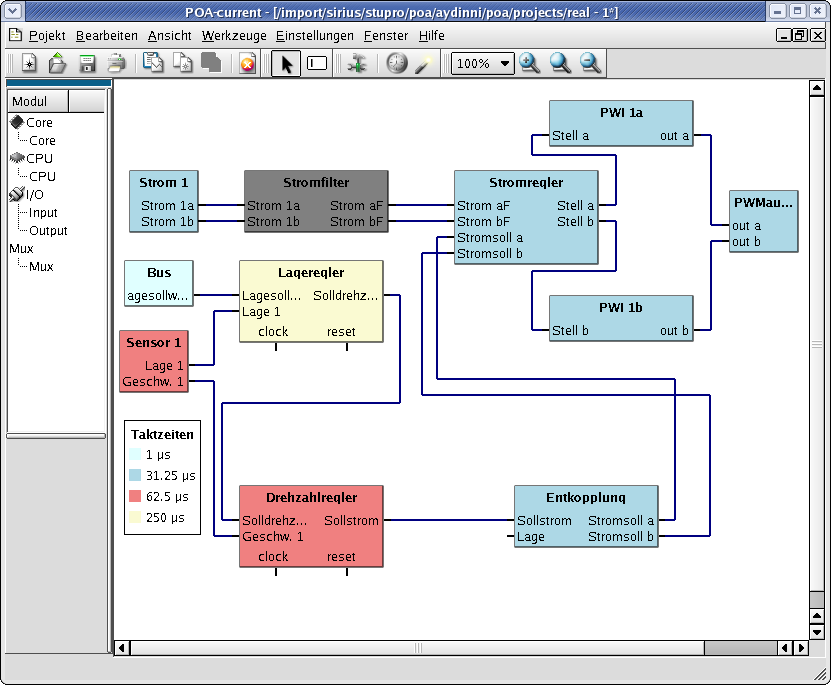
\includegraphics[width=15cm]{Mainwindow1}

\caption{Mainwindow}\label{test}

\end{center}

\end{figure}

Die Men"uleiste besteht aus den Men"us Project, Edit, View, Tools, Settings, Windows und Help.\par
\newpage
Die hier Kurz beschriebenen Funktionen werden in den folgenden Abschnitten n"aher erkl"art.\par

\begin{itemize}
\item {\bf Project:}	New, Open, Save, Save as, Print, Recent, Exit\newline
Unter Project hat man die M"oglichkeit Projekte anzulegen, zu "offnen, abzuspeichern, auszudrucken und POA zu beenden.
\item {\bf Edit:}	Cut, Copy, Paste\newline
Unter diesem Men"upunkt kann man die Aktionen Ausschneiden, Kopieren und Einf"ugen ausf"uhren.
\item {\bf View:}	Zoom in, Zoom normal, Zoom out\newline
Unter View ist es m"oglich den Inhalt im Arbeitsfenster an- und auszuzoomen.
\item {\bf Tools:} 	Configuration, Route, Scheduling, Deploy Project\newline
Unter Tools k"onnen markierte Bl"ocke konfiguriert oder markierte Verbindungen geroutet werden. Au"serdem kann man hier im Untermen"u Scheduling den Ablauf f"ur die Bl"ocke graphisch darstellen und manipulieren. Das Untermen"u Deploy Project bietet die M"oglichkeit am Projekt ein Konsistenzcheck durchzuf"uhren, den CPU-Prgrammcode zu kompilieren und es auf das CPLD-Board herunterzuladen.
\item {\bf Settings:}	Show Grid, Configure POA\newline
Unter Settings k"onnen Grundeinstellungen an POA vorgenommen werden. Hier kann z.B. das Raster, die Programmsprache eingestellt und externe Tools (Editor, Compiler, ...) eingebunden werden.
\item {\bf Windows:} 	Tile, Tile Horizontal, Cascade\newline
Hier k"onnen, falls mehrere Projekte gleichzeitig ge"offnet sind, die Arbeitsfenster je nach Wunsch nebeneinander, "ubereinander oder kaskadiert angezeigt werden.
\item {\bf Help:} 	Contens, About\newline
Unter Help finden allgemeine Informationen "uber POA.\par
\end{itemize}

Die wichtigsten Aktionen k"onnen auch mit den Befehlsbuttons in der Symbolleiste oder im Kontextmen"u beim Markieren mit der rechten Maustaste ausgew"ahlt werden.

%\section{Dailogen}
%
%\subsubsection{POA Konfiguration Dailog}
%In diesem Konfigurationsdialog k"onnen alle m"oglichen Softwareeinstellungen vorgenommen %werden.
%\begin{figure}[htbp]
%\begin{center}
%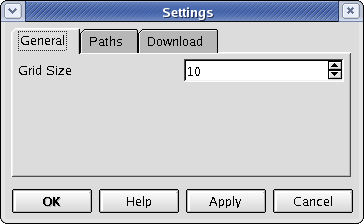
\includegraphics[width=10cm]{POAConfiguration1}
%\caption{POA Configuration}\label{test}
%\end{center}
%\end{figure}
%
%\subsubsection{Block Konfiguration Dailog}
%In diesem Konfigurationsdialog k"onnen die Bl"ocke (CPUs, Cores, Input-Block,
%Output-Block, Mux-Block) so konfiguriert werden, dass sie mit dem vorgegebenen
%CPLD-Design "ubereinstimmen.
%\begin{figure}[htbp]
%\begin{center}
%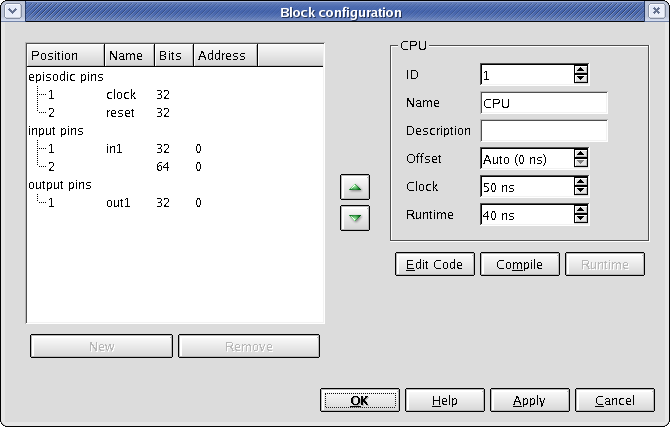
\includegraphics[width=10cm]{CPUConfiguration}
%\caption{Block Configuration}\label{test}
%\end{center}
%\end{figure}
%
%\subsubsection{Scheduling Dailog}
%In diesem Dialog werden Laufzeit, Takt und Offset der Bl"ocke visuell dargestellt. "Uber den %Offset der Bl"ocke kann eine Optimierung des CPLDs angestrebt werden.
%\begin{figure}[htbp]
%\begin{center}
%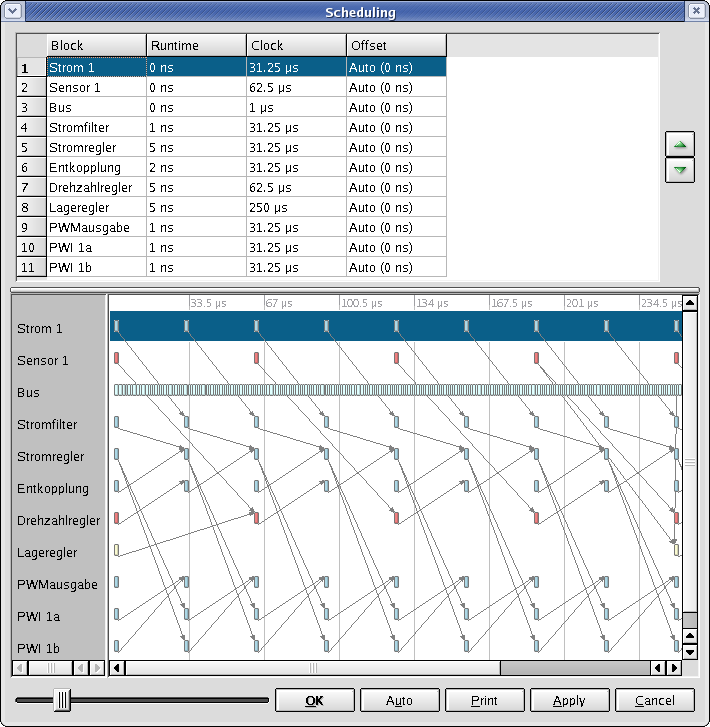
\includegraphics[width=10cm]{Scheduling1}
%\caption{Scheduling}\label{test}
%\end{center}
%\end{figure}
%
%\subsubsection{Wizard Dailog}


%%%%%%%%%%%%%%%%%%%%%%%%%%%%%%%%%%%%%%%%%%%%%%%%%%%%%%%%%%%%%%%%%%%%%%%%%%%%%
%%%%%%%%%%%%%%%%%%%%%%%%%%%%%%%%%%%%%%%%%%%%%%%%%%%%%%%%%%%%%%%%%%%%%%%%%%%%%

\chapter{Referenz}

\section{Allgemein}
\subsection{Farbgebung}
POA bietet durch die F"arbung der Bl"ocke nach Ihrer Taktzahl eine komfortabele "Ubersicht "uber die Bl"ocke. D.h. gleichgetaktete Bl"ocke werden auch in der gleiche Farbe angezeigt.\newline
In der {\bf Takttabelle}, standardm"a"sig im oberen linken Rand des Layouts, sind die Farben und die dazugeh"origen Taktzeiten aufgelistet. Die {\bf Takttabelle} kann frei verschoben werden, indem man die Tabelle mit der linken Maustaste ausw"ahlt und mit gedr"uckter Taste den Mauszeiger im Arbeitsfenster bewegt.\par
Markierte Objekte werden immer grau angezeigt.\newline
Verbindungen werden immer blau gezeichnet, es sei denn es besteht ein Konflikt zwischen den Pins. Dann wird die Verbindung rot markiert.


\subsection{Tooltip}
Mit der Tooltipfunktion bietet POA eine komfortabele L"osung, um Kurzinformationen "uber die Objekte im Arbeitsfenster zu erhalten. Um eine Tooltipinformation von einer Verbindung oder einem Block zu erhalten, muss man mit dem Mauszeiger auf das Objekt zeigen. Nach kurzer Zeit erscheint dann die Tooltipinformation in Form eines gelben K"astchens.

%%%%%%%%%%%%%%%%%%%%%%%%%%%%%%%%%%%%%%%%%%%%%%%%%%%%%%%%%%%%%%%%%%%%%%%%%%%%%
\subsection{Beschriftung des Layouts}
\subsubsection{Layoutbeschriftung setzen}
Um im Layout Beschriftungen (z.B. Kommentare) vorzunehmen, muss man mit dem Mauszeiger auf das Symbol {\bf Annotate} in der Symbolleiste klicken.% Alternativ kann man auch mit linken Maustaste ins Arbeitsfenster klicken und im Kontextme"u den Eintrag {\bf Annotate} w"ahlen.%
Der Mauszeiger wird zu einem Cursor, den man nun frei im Arbeitsfenster positionieren kann. Klickt man mit dem Cursor an die Stelle, wo die Beschriftung hin soll, wird ein Dialog mit einem Textfeld "offnet, in den man den gew"unschten Text eingeben kann. Bei Best"atigung mit {\bf OK} wird der Dialog geschlossen und der Text wird an die gew"unschte Stelle gesetzt.\par
Um dem Cursormodus verlassen zu k"onnen, muss man nur das Symbol {\bf Mauszeiger} in der Symbolleiste anklicken.
\subsubsection{Layoutbeschriftung verschieben}
Zum Verschieben der Layoutbeschriftung, muss man die Beschriftung mit der linken Maustaste ausw"ahlen und die Taste dabei gedr"uckt lassen. Jetzt kann man die Layoutbeschriftung frei im Arbeitsfenster auf die gew"unschte Position verschieben. Beim Loslassen der Maustaste wird die Beschriftung an diese Stelle gesetzt.
\subsubsection{Layoutbeschriftung l"oschen}
Um eine Beschriftung im Layout zu l"oschen, muss man den zu l"oschenden Text im Layout mit der rechten Maustaste ausw"ahlen und im Kontextmen"u den Eintrag {\bf Remove} w"ahlen. Altenativ kann man auch das Symbol {\bf Remove} in der Symbolleiste anklicken.
Dabei wird die Beschriftung an dieser Stelle unwiderruflich gel"oscht.

%%%%%%%%%%%%%%%%%%%%%%%%%%%%%%%%%%%%%%%%%%%%%%%%%%%%%%%%%%%%%%%%%%%%%%%%%%%%%

\subsection{Zoomen}
Mit der Zoomfunktion hat man die M"oglichkeit das Layout heran- oder wegzuzommem. POA unterst"utzt das Zoomen zwischen 10{\%} und 500{\%}. Die Standardeinstellung, d.h. die Normalansicht, ist bei einem Zoomfaktor von 100\%.\newline
Zum "Andern des Zoomfaktors, kann man entweder die Zoomsymbole in der Symbolleiste oder die Eintr"age im Men"u {\bf View} w"ahlen.

%%%%%%%%%%%%%%%%%%%%%%%%%%%%%%%%%%%%%%%%%%%%%%%%%%%%%%%%%%%%%%%%%%%%%%%%%%%%%

\subsection{Die Standard Button}
\begin{figure}[htbp]

\begin{center}

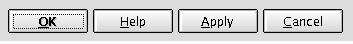
\includegraphics[width=10cm]{Button}

\caption{Tasten}\label{test}

\end{center}

\end{figure}
Mit {\bf OK} werden die Einstellungen f"ur das Projekt gespeichert und der Dialog wird geschlossen.\par
Mit {\bf Apply} werden die Einstellungen "ubernommen.\par
Mit {\bf Cancel} werden die Einstellungen verworfen und der Dialog wird geschlossen.\par
Die Taste {\bf Help} ist in dieser Version von POA nicht belegt.


%%%%%%%%%%%%%%%%%%%%%%%%%%%%%%%%%%%%%%%%%%%%%%%%%%%%%%%%%%%%%%%%%%%%%%%%%%%%%
%%%%%%%%%%%%%%%%%%%%%%%%%%%%%%%%%%%%%%%%%%%%%%%%%%%%%%%%%%%%%%%%%%%%%%%%%%%%%
\newpage
\section{POA konfigurieren}

\subsection{Raster einstellen}
\begin{figure}[htbp]

\begin{center}

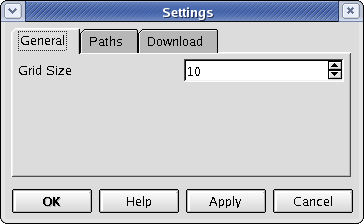
\includegraphics[width=10cm]{POAConfiguration1}

\caption{POA Konfiguration}\label{test}

\end{center}

\end{figure}
Die Bl"ocke und Verbindungen richten sich im Arbeitsfenster einem vorgegebenen Raster aus.\par

Zur Ver"anderung der Rastergr"o"se muss man im Untermen"u von {\bf Settings} den Eintrag {\bf Configure POA} ausw"ahlen. Im aufklappenden Dialog kann man unter dem Dateireiter {\bf General} die gew"unschte Rastergr"o"se eingeben.\par
Man kann das Raster anzeigen lassen oder ausblenden. Dazu w"ahlt man im Untermen"u von {\bf Settings} den Eintrag {\bf Show Grid} oder man dr"uckt die rechte Maustaste und w"ahlt {\bf Show Grid} im Kontextmen"u.


%%%%%%%%%%%%%%%%%%%%%%%%%%%%%%%%%%%%%%%%%%%%%%%%%%%%%%%%%%%%%%%%%%%%%%%%%%%%%
\subsection{Sprache einstellen}
POA unterst"utzt die Sprachen Deutsch und Englisch.\par
Zur Ver"anderung der Sprache muss man im Untermen"u von {\bf Settings} den Eintrag {\bf Configure POA} ausw"ahlen. Im aufklappenden Dialog kann man unter dem Dateireiter {\bf General} in der Auswahlbox {\bf Language} zwischen Englisch und Deutsch w"ahlen. Die "Anderungen bez"uglich der Sprachauswahl werden erst bei einem Neustart von POA wirksam.\par

%%%%%%%%%%%%%%%%%%%%%%%%%%%%%%%%%%%%%%%%%%%%%%%%%%%%%%%%%%%%%%%%%%%%%%%%%%%%%
\subsection{Externe Programme einbinden}
POA bietet die M"oglichkeit externe Programme einzubinden und sie direkt und komfortabel aus POA heraus zu starten. Mit einem Editor kann der Quellcode f"ur die CPU in der Programmiersprache C  verfasst werden. Zum Kompilieren ben"otigt POA einen C-Compiler und f"ur das Herunterladen des kompilierten Quellcodes auf die CPLD wird ein Download Tool ben"otigt.\par
Zur Einbindung der externen Programme muss man im Untermen"u von {\bf Settings} den Eintrag {\bf Configure POA} w"ahlen. Im aufklappenden Dialog kann man unter dem Dateireiter {\bf Paths} die gew"unschten Programme einbinden.

\begin{figure}[htbp]

\begin{center}

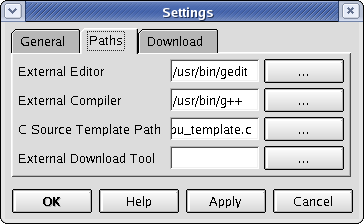
\includegraphics[width=10cm]{POAConfiguration2}

\caption{POA Konfiguration}\label{test}

\end{center}

\end{figure}

\subsubsection{Externen Editor einbinden}
Um einen Editor einzubinden, w"ahlt man unter dem Dateireiter {\bf Paths} das Textfeld neben {\bf External Editor} aus und gibt hier den korrekten Pfad des Editors ein. Alternativ dazu kann man auch mit dem Button neben dem Textfeld im Verzeichnisbaum nach dem gew"unschten Editor suchen.\par
\subsubsection{Externen Compiler einbinden}
Um einen Compiler einzubinden, w"ahlt man unter dem Dateireiter {\bf Paths} das Textfeld neben {\bf External Compiler} aus und gibt hier den korrekten Pfad des Compilers ein. Alternativ dazu kann man auch mit dem Button neben dem Textfeld im Verzeichnisbaum nach dem gew"unschten Compiler suchen.\par
\subsubsection{Externen Download Tool einbinden}
Um einen Download Tool einzubinden, w"ahlt man unter dem Dateireiter {\bf Paths} das Textfeld neben {\bf External Download Tool} aus und gibt hier den korrekten Pfad des Download Tool ein. Alternativ dazu kann man auch mit dem Button neben dem Textfeld im Verzeichnisbaum nach dem gew"unschten Download Tool suchen. \par



%%%%%%%%%%%%%%%%%%%%%%%%%%%%%%%%%%%%%%%%%%%%%%%%%%%%%%%%%%%%%%%%%%%%%%%%%%%%%
\newpage
\subsection{C Source Template Pfad angeben}
Mit dem C Source Template wird der Rahmencode f"ur den Quellcode der CPU vorgegeben.
Um einen C Source Template Pfad anzugeben, w"ahlt man unter dem Dateireiter {\bf Paths} das Textfeld neben {\bf C Source Template Path} aus und gibt hier das korrekte Verzeichnis an. Alternativ dazu kann man auch mit dem Button neben dem Textfeld im Verzeichnisbaum nach dem gew"unschten Pfad suchen. \par


%%%%%%%%%%%%%%%%%%%%%%%%%%%%%%%%%%%%%%%%%%%%%%%%%%%%%%%%%%%%%%%%%%%%%%%%%%%%%
\subsection{Download Einstellung}
\begin{figure}[htbp]

\begin{center}

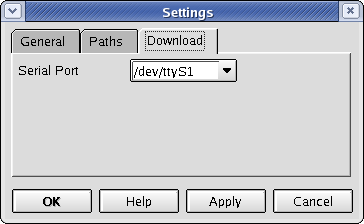
\includegraphics[width=10cm]{POAConfiguration3}

\caption{POA Konfiguration}\label{test}

\end{center}

\end{figure}
F"ur Downloadeinstellungen w"ahlt man den Dateireiter {\bf Download}. Hier kann man in der Auswahlbox den Seriellen Port, an dem das CPLD-Board angeschlossen ist, einstellen.\par


%%%%%%%%%%%%%%%%%%%%%%%%%%%%%%%%%%%%%%%%%%%%%%%%%%%%%%%%%%%%%%%%%%%%%%%%%%%%%
%%%%%%%%%%%%%%%%%%%%%%%%%%%%%%%%%%%%%%%%%%%%%%%%%%%%%%%%%%%%%%%%%%%%%%%%%%%%%
\newpage
\section{Ein Projekt anlegen, "offnen, speichern}
\begin{figure}[htbp]

\begin{center}

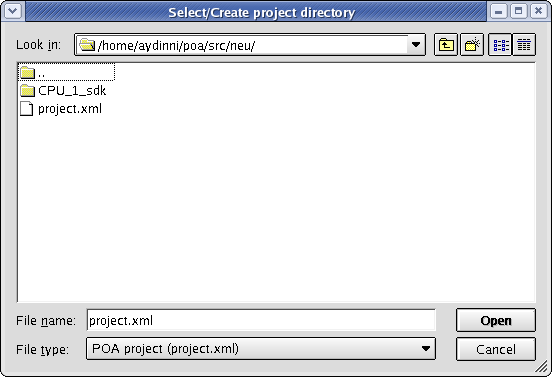
\includegraphics[width=10cm]{Directory}

\caption{Project Directory}\label{test}

\end{center}

\end{figure}

\subsection{Neues Projekt anlegen}
Durch Anklicken des Men"us {\bf Project} in der Men"uleiste erscheint ein Untermen"u {\bf New}. Wenn dies ausgew"ahlt oder altenativ dazu mit der Maus auf das Symbol {\bf New} in der Symbolleiste geklickt wird, wird ein Dailog ge"offnet, in dem man das Verzeichnis f"ur das neue Projekt anlegen kann. Dazu kann man im Verzeichnisbaum das Verzeichnis suchen, in dem der Zielordner angelegt wird. Zum Erstellen des Zielordners klickt man auf das Symbol {\bf Create New Folder}. Dabei wird ein neuer Ordner angelegt, dem nun ein Name vergeben werden kann. Um das neue Projekt hier anzulegen, muss man den Zielordner "offnen und auf {\bf OK} klicken.\newline
Es kann nur ein Projekt pro Verzeichnis angelegt werden.\par
Wird ein neues Projekt angelegt, dann wird dadurch auch das Arbeitsfenster im Hauptfenster aktiviert.


%%%%%%%%%%%%%%%%%%%%%%%%%%%%%%%%%%%%%%%%%%%%%%%%%%%%%%%%%%%%%%%%%%%%%%%%%%%%%
\subsection{Bestehendes Projekt "offnen}
Im Untermen"u von {\bf Project} den Eintrag {\bf Open} oder in der Symbolleiste den {\bf Ordner} anklicken. Im nun aufklappendem Dialog kann man im Verzeichnisbaum das gew"unschte Projekt (project.xml-Datei) suchen und mit einem Doppelklick auf die Datei oder mit dem {\bf Open} Button "offen.
Im Arbeitsfenster erscheint nun das Projekt mit den Funktionsbl"ocken (CPUs, Cores,..) und den Verbindungen, d.h. dem Vernetzungsplan.\par


%%%%%%%%%%%%%%%%%%%%%%%%%%%%%%%%%%%%%%%%%%%%%%%%%%%%%%%%%%%%%%%%%%%%%%%%%%%%%
\subsection{Projekt speichern}
Im Untermen"u von {\bf Project} den Eintrag {\bf Save} oder in der Symbolleiste die {\bf Diskette} anklicken. Dabei wird das Projekt automatisch in das urspr"ungliche Verzeichnis gespeichert.\par
Mit dem Eintrag {\bf Save as} kann das Projekt in ein anderes Verzeichnis gespeichert werden. Dabei wird ein Dialog ge"offnet, in den man das Verzeichnis angeben kann.\par


%%%%%%%%%%%%%%%%%%%%%%%%%%%%%%%%%%%%%%%%%%%%%%%%%%%%%%%%%%%%%%%%%%%%%%%%%%%%%
%%%%%%%%%%%%%%%%%%%%%%%%%%%%%%%%%%%%%%%%%%%%%%%%%%%%%%%%%%%%%%%%%%%%%%%%%%%%%
\section{Layout drucken}
\begin{figure}[htbp]

\begin{center}

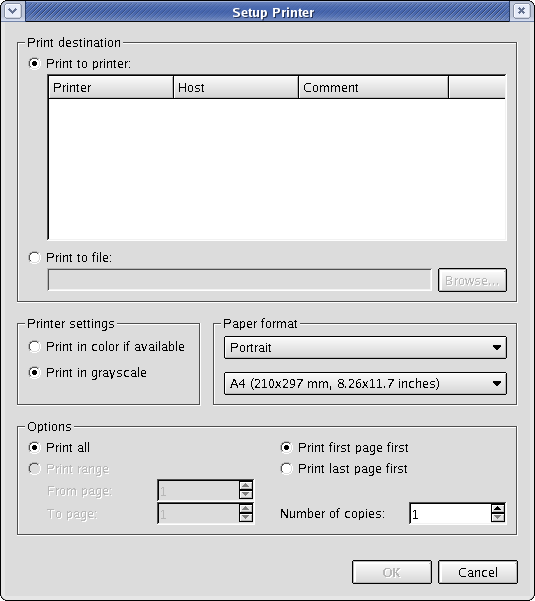
\includegraphics[width=10cm]{Printer}

\caption{Setup Printer}\label{test}

\end{center}

\end{figure}
POA bietet die M"oglichkeit das entworfene Layout und die graphische Darstellung des Scheduling zu drucken oder als druckbare Datei zu speichern.
Dazu kann man im Untermen"u {\bf Project} den Eintrag {\bf Print} oder in der Symbolleiste den {\bf Drucker} w"ahlen. Im nun aufklappendem Dialog kann man die gew"unschten Druckeinstellungen vornehmen und den Druckauftrag an den ausgew"ahlten Drucker mit der Best"atigung durch {\bf OK} schicken.\par
Mit {\bf Cancel} werden die Einstellungen verworfen.\par






%%%%%%%%%%%%%%%%%%%%%%%%%%%%%%%%%%%%%%%%%%%%%%%%%%%%%%%%%%%%%%%%%%%%%%%%%%%%%
%%%%%%%%%%%%%%%%%%%%%%%%%%%%%%%%%%%%%%%%%%%%%%%%%%%%%%%%%%%%%%%%%%%%%%%%%%%%%
\newpage
\section{Bl"ocke}

\subsection{Bl"ocke erzeugen}
Bl"ocke, wie CPUs, Cores etc. k"onnen per Drag`n Drop aus der Blockbibliothek in das Arbeitsfenster gezogen werden und dadurch erzeugt werden. Wenn man ein Block ins Arbeitsfenster gezogen hat und die Maustaste wieder losl"a"st, wird automatisch das Konfigurationsfenster f"ur den Block ge"offnet. Hier hat man die M"oglichkeit verschiedene Einstellungen vornehmen.

%%%%%%%%%%%%%%%%%%%%%%%%%%%%%%%%%%%%%%%%%%%%%%%%%%%%%%%%%%%%%%%%%%%%%%%%%%%%%
\subsection{Blockkonfiguration allgemein}
Beim Erzeugen eines Blocks wird ein Konfigurationsdialog automatisch ge"offnet. Hier hat man je nach Block verschiedene Konfigurationsm"oglichkeiten. Der Konfigurationsdialog kann auch sp"ater ge"offnet werden. Dazu w"ahlt man den zu konfigurierenden Block mit der rechten Maustaste aus und w"ahlt im Kontextmen"u den Eintrag {\bf Configuration}, oder man f"uhrt ein Doppelklick mit der linken Maustaste auf den Block aus.\par
Alternativ dazu kann man f"ur den ausgew"ahlten Block die Funktion auch "uber die Men"uleiste oder Symbolleiste ausf"uhren. \par

\begin{figure}[htbp]

\begin{center}

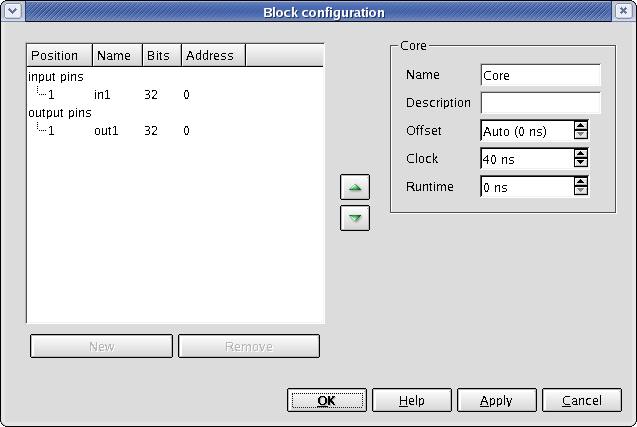
\includegraphics[width=10cm]{CoreBlockConfiguration}

\caption{Block Konfiguration}\label{test}

\end{center}

\end{figure}

\subsubsection{Blockname "andern}
Zur eindeutigen Identifizierung der Bl"ocke ist es von Vorteil den Bl"ocken einen aussagekr"aftigen Namen zu geben. Aussagekr"aftige Namen sorgen auch daf"ur, dass man sofort wei"s, wof"ur ein Block gut ist. \par
Im Textfeld {\bf Name} kann man den neuen Namen des Blocks eingeben.
\subsubsection{Block beschreiben}
Im Textfeld {\bf Description} kann man Beschreibungen oder Komentare zum Block eingeben. Diese erscheinen im Tooltip, wenn man mit dem Mauszeiger auf den Block zeigt oder im der Infobox, wenn der Block in die Blockbibliothek aufgenommen ist.\par
Die Blockbeschreibung hat den Vorteil, dass man sp"ater auch noch leicht nachvollziehen kann, wasf"ur Eigenschaften dieser Block hat.\par
Diese Option ist f"ur {\bf Multiplexer} nicht verf"ugbar.
\subsubsection{Neue Pins erzeugen}
In der Pinbibliothek k"onnen blockabh"angig drei verschiedene Arten von Pins ("'Episodic Pin"', "'Input Pin"' und "'Output Pin"') verwaltet werden. Je nach Pinart w"ahlt man in der Bibliothek die entsprechende Kategorie. Dabei wird der {\bf New} Button aktiviert. Mit einem Klick auf den aktivierten {\bf New} Button wird ein neuer Pin erzeugt. \par
\subsubsection{Pins l"oschen}
Dazu w"ahlt man in der Pinbibliothek den zu l"oschende Pin aus. Der {\bf Remove} Button wird nun aktiviert. Mit einem Mausklick auf den {\bf Remove} Button wird der Pin gel"oscht. Wenn an diesem Pin eine Verbindung angedockt war, wird diese Verbindung automatisch mitgel"oscht.
\subsubsection{"Anderungen an Pins vornehmen}
Dazu w"ahlt man in der Pinbibliothek den zu "andernde Pin aus.\par
Unter der Spalte {\bf Name} kann man dem Pin einen Namen geben oder einen vorhandenen Namen "andern.\par
Unter der Spalte {\bf Bits} kann die Anzahl der Bits, d.h. die Bitbreite, f"ur ein Pin ge"andert werden. Es ist m"oglich eine Bitbreite von 0 bis 64 anzugeben.\par
Unter der Spalte {\bf Address} kann eine Adressierung f"ur die Input-Pins und Output-Pins vornehmen werden.\par
\subsubsection{Offset eingeben}
Der Offset ist f"ur das Scheduling, d.h. f"ur die Optimierung der Gesamtlaufzeit, wichtig. Die Offsetzeit ist diejenige Zeit, mit der ein Block versp"atet gestartet wird.
Um den Offset an einem Block anzugeben, kann man entweder direkt mit der Maus ins Textfeld {\bf Offset} klicken und die Offsetzeit dort in Nanosekunden eingeben oder man benutzt die Pfeiltasten neben dem Textfeld.\par
Diese Option ist f"ur {\bf Multiplexer} nicht verf"ugbar.
\subsubsection{Takt eingeben}
Um die Taktrate eines Blocks anzugeben, kann man entweder direkt mit der Maus ins Textfeld {\bf Clock} klicken und die Taktfrequenz dort in Nanosekunden eingeben oder man benutzt die Pfeiltasten neben dem Textfeld.\par
Diese Option ist f"ur {\bf Multiplexer} nicht verf"ugbar.
\subsubsection{Laufzeit eingeben}
Um die Laufzeit eines Blocks anzugeben, kann man entweder direkt mit der Maus ins Textfeld{\bf Runtime} klicken und die Laufzeit dort in Nanosekunden eingeben oder man benutzt die Pfeiltasten neben dem Textfeld.\par
Diese Option ist f"ur {\bf Multiplexer} und {\bf Inputbl"ocke} nicht verf"ugbar.


%%%%%%%%%%%%%%%%%%%%%%%%%%%%%%%%%%%%%%%%%%%%%%%%%%%%%%%%%%%%%%%%%%%%%%%%%%%%%
\subsection{I/O Block konfigurieren}
Siehe Kapitel {\bf Blockkonfiguration allgemein}.

%\begin{figure}[htbp]
%\begin{center}
%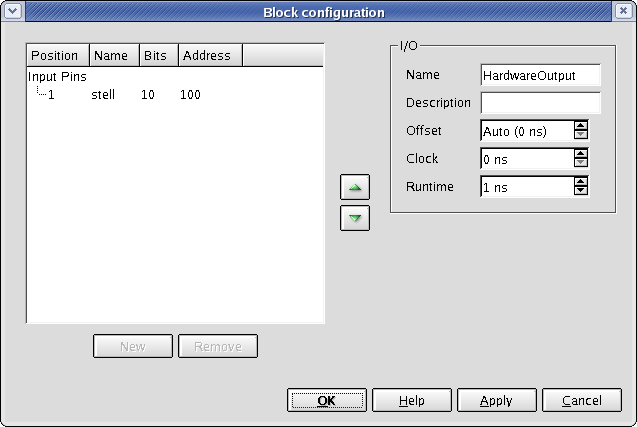
\includegraphics[width=10cm]{OutputBlockConfiguration}
%\caption{I/O Block Configuration}\label{test}
%\end{center}
%\end{figure}


%%%%%%%%%%%%%%%%%%%%%%%%%%%%%%%%%%%%%%%%%%%%%%%%%%%%%%%%%%%%%%%%%%%%%%%%%%%%%
\subsection{Core konfigurieren}
Siehe Kapitel {\bf Blockkonfiguration allgemein}.

\newpage
%%%%%%%%%%%%%%%%%%%%%%%%%%%%%%%%%%%%%%%%%%%%%%%%%%%%%%%%%%%%%%%%%%%%%%%%%%%%%
\subsection{CPU konfigurieren}
\begin{figure}[htbp]

\begin{center}

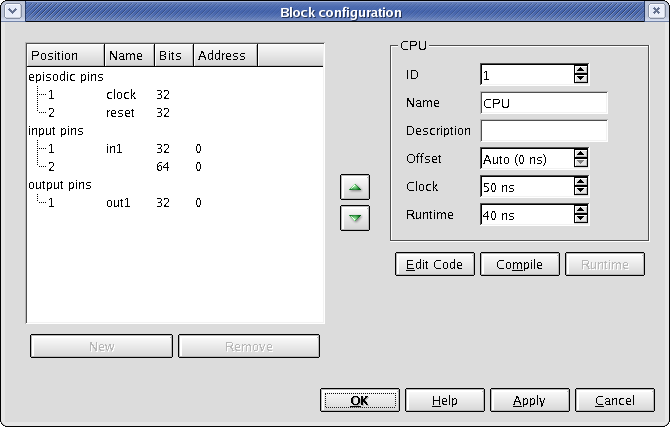
\includegraphics[width=10cm]{CPUConfiguration}

\caption{CPU Konfiguration}\label{test}

\end{center}

\end{figure}
\subsubsection{ID eingeben}
Jeder CPU muss eine ID (d.h. eine Nummer von 0 - 99) vergeben werden, dazu kann man entweder direkt mit der Maus ins Textfeld {\bf ID} klicken und die Nummer eingeben oder man benutzt die Pfeiltasten neben dem Textfeld. Falls eine schon vergebene ID ausgew"ahlt wird, erscheint rechts neben dem Textfeld {\bf ID} ein Warnsignal.

\subsubsection{Die CPU-Programmcode schreiben}
Zum Schreiben von CPU-Programmcode wird ein externer Editor aufgerufen, wenn im Konfigurationsdialog der Button {\bf Edit Code} gedr"uckt wird. Beim "Offnen des des Editors wird automatisch ein C-Source Template geladen, der einen generierten Rahmencode f"ur die CPU in der Programmiersprache C vorgibt. Im Editor kann dann der restliche Quellcode f"ur die CPU niederschreiben und abspeichern.

\newpage
\subsubsection{CPU-Programmcode kompilieren}
Zum Kompilieren des erzeugten CPU-Programmcodes wird ein externer Compiler gestartet, wenn im Konfigurationsdialog der Button {\bf Compile} gedr"uckt wird. Der Compiler kompiliert den CPU-Programmcode und gibt im {\bf POA Terminal} eine entsprechende Meldung aus.

\begin{figure}[htbp]

\begin{center}

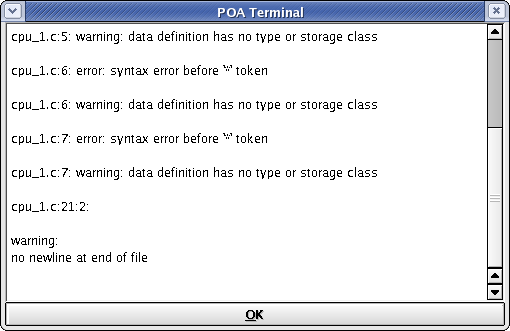
\includegraphics[width=10cm]{Terminal}

\caption{POA Terminal}\label{test}

\end{center}

\end{figure}




%%%%%%%%%%%%%%%%%%%%%%%%%%%%%%%%%%%%%%%%%%%%%%%%%%%%%%%%%%%%%%%%%%%%%%%%%%%%%
\newpage
\subsection{Multiplexer konfigurieren}
\begin{figure}[htbp]

\begin{center}

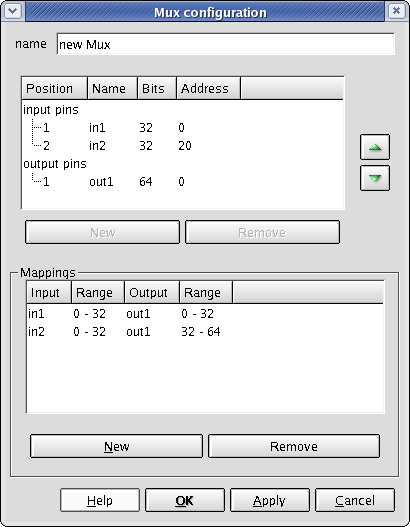
\includegraphics[width=10cm]{MuxConfiguration}

\caption{Multiplexer Konfiguration}\label{test}

\end{center}

\end{figure}

Multiplexer dienen dazu mehrere Eingangssignale auf ein Ausgangssignal zu reduzieren oder umgekehrt ein  Eingangssignal auf mehrere Ausgangssignale zu verteilen.
Im {\bf Mapping}Bereich des Konfigurationsdialogs wird die aktuelle Zuordnung der Bits des Eingangspins auf die des Ausgangspins angezeigt.\par
Um eine neue Zuordnung zu erstellen, muss man auf den Button {\bf New} klicken. Dabei wird ein neuer Dialog ge"offnet. In diesem Dialog (Mux mapping configuration) hat man die M"oglichkeit den Eingangsbits bestimmte Ausgangsbits zuzuordnen. Dazu w"ahlt man in der Auswahlbox {\bf Input} den Eingangspin und in der Auswahlbox {\bf Output} den Ausgangspin des Multiplexers. In den Textfeldern {\bf first bit} und {\bf last bit} kann die Zuordnung zwischen Eingangsbits und Ausgangsbits vorgenommen werden.\par

Um eine vorhandene Zuordnung zu ver"andern, muss der entsprechende Eintrag in der Mappingtabelle markiert werden. Dabei werden die Buttons {\bf Update} und {\bf Remove} aktiviert.\newline
Mit {\bf Update} wird der Dialog {\bf Mux mapping configuration} ge"offnet. Hier kann man wie oben beschrieben, die "Anderungen in der Zuordnung vornehmen.\newline

\begin{figure}[htbp]

\begin{center}

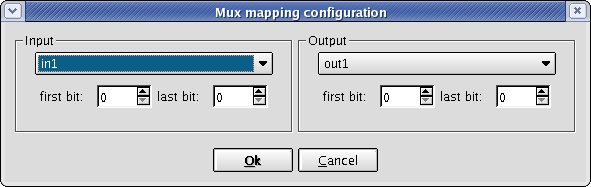
\includegraphics[width=10cm]{Muxzuordnung}

\caption{Mux mapping configuration}\label{test}

\end{center}

\end{figure}

Mit {\bf Remove} kann man die ausgew"ahlte Zuordnung l"oschen.\par


%%%%%%%%%%%%%%%%%%%%%%%%%%%%%%%%%%%%%%%%%%%%%%%%%%%%%%%%%%%%%%%%%%%%%%%%%%%%%
\subsection{Blockbibliothek}
Die Blockbibliothek verwaltet standardm"a"sig die von POA vorgegeben Standardbl"ocke.
Bl"ocke, die einmal konfiguriert worden sind und oft wiederverwendet werden sollen, 
k"onnen in der Blockbibliothek auch verwaltet werden. Dadurch wird die Wiederverwendung
von Bl"ocken erleichtert und die Bl"ocke f"ur andere Projekte zur Verf"ugung gestellt.\par
In der Infobox unter der Blockbibliothek werden Informationen zu den ausgew"ahlten Bl"ocken aus der Bibliothek angezeigt. Die Informationen kommen aus der Beschreibung der Bl"ocke, welche bei der Blockkonfiguration eingetragen worden sind.
\subsubsection{Block in die Blockbibliothek aufnehmen}
Um ein Block in die Bibliothek aufzunehmen, klickt man mit der rechten Maustaste
auf den Block und w"ahlt im Kontextmen"u den Eintrag {\bf Save To Library}. Je nach Art des Blocks kann man den Block in die entsprechende Kategorie setzten. Dazu w"ahlt man im ge"offneten Dialog den Blocktyp in der Auswahlbox aus. Nach den Best"atigen mit {\bf OK}, wird dieser Block in der Blockbibliothek aufgenommen.\newline
Bl"ocke, die in die Bibliothek aufgenommen werden, werden projektunabh"angig gespeichert
und stehen bei jedem Neustart von POA zur Verf"ugung.
\subsubsection{Blocktyp in der Blockbibliothek "andern}
Dazu muss man den Block in der Bibliothek mit der rechten Maustaste markieren und im Kontextmen"u den Eintrag {\bf Change Type} w"ahlen. Im geo"ffneten Dialog kann man in der Auswahlbox den gew"unschten Blocktyp ausw"ahlen und mit {\bf OK} best"atigen. Der Block wird nun in die gew"unschten Kategorie verschoben.
\subsubsection{Block in der Blockbibliothek umbenennen}
Dazu muss man den Block in der Bibliothek mit der rechten Maustaste markieren und im Kontextmen"u den Eintrag {\bf Rename} w"ahlen. Der nun gehighlightete Name kann "uberschrieben und mit der Eingabebest"atigung gespeichert werden.
\subsubsection{Block aus der Blockbibliothek entfernen}
Bl"ocke k"onnen auch wieder aus der Bibliothek entfernt werden. Dazu muss man den
Block in der Bibliothek mit der rechten Maustaste markieren und im Kontextmen"u den
Eintrag {\bf Remove} w"ahlen. Der ausgew"ahlte Block wird dabei unwiderruflich aus der Blockbibliothek entfernt.

%%%%%%%%%%%%%%%%%%%%%%%%%%%%%%%%%%%%%%%%%%%%%%%%%%%%%%%%%%%%%%%%%%%%%%%%%%%%%
\subsection{Block in Arbeitsfenster verschieben}
Zum Verschieben eines Blocks, w"ahlt man den Block mit der linken Maustaste aus, l"a"st die Taste gedr"uckt und verschiebt den Block in Arbeitsfenster bis man die gew"unschte Position hat. Dabei werden die Verbindungen, die an diesem Block h"angen automatisch mitgeroutet.


%%%%%%%%%%%%%%%%%%%%%%%%%%%%%%%%%%%%%%%%%%%%%%%%%%%%%%%%%%%%%%%%%%%%%%%%%%%%%
\subsection{Block kopieren und einf"ugen}
Wenn man mehrere identische Bl"ocke f"ur das Layout in einem oder in verschiedenen Projekten ben"otigt, eignet sich dazu die "'copy and paste"' Funktion. Hierzu w"ahlt man den Block mit der rechten Maustaste aus. Im Kontextmen"u w"ahlt man den Eintrag {\bf Copy}. Wenn man nun mit der linken Maustaste auf ein freies Feld im Arbeitsfenster klickt, kann man im Kontextmen"u den Eintrag {\bf Paste} w"ahlen, um eine Kopie des ausgew"ahlten Blocks zu erzeugen.
Die Kopie wird automatisch im linken oberen Rand des Arbeitsfensters positioniert.\newline
Alternativ kann diese Aktion auch "uber die Men"uleiste bzw. Symbolleiste ausgef"uhrt werden.


%%%%%%%%%%%%%%%%%%%%%%%%%%%%%%%%%%%%%%%%%%%%%%%%%%%%%%%%%%%%%%%%%%%%%%%%%%%%%
\subsection{Block ausschneiden und einf"ugen}
Hierbei geht man wie zuvor im Abschnitt "'Block kopieren und einf"ugen"' vor, mit der Ausnahme, dass statt der Aktion {\bf Copy} die Aktion {\bf Cut} w"ahlt wird. \par
Wenn ein Block ausgeschnitten wird, werden alle Verbindungen zu diesem Block unwiderruflich gel"oscht.


%%%%%%%%%%%%%%%%%%%%%%%%%%%%%%%%%%%%%%%%%%%%%%%%%%%%%%%%%%%%%%%%%%%%%%%%%%%%%
\subsection{Block l"oschen}
Um ein Block zu l"oschen, w"ahlt man den Block mit der rechten Maustaste aus. Im Kontextmen"u wird der Eintrag {\bf Remove} aktiv. Bei Auswahl von {\bf Remove} wird der Block unwiderruflich gel"oscht.\newline
Altenativ kann f"ur den ausgew"ahlten Block diese Aktion auch "uber die Men"uleiste bzw. Symbolleiste ausgef"uhrt werden.\newline
Wenn ein Block gel"oscht wird, werden alle Verbindungen zu diesem Block auch unwiderruflich gel"oscht.


%%%%%%%%%%%%%%%%%%%%%%%%%%%%%%%%%%%%%%%%%%%%%%%%%%%%%%%%%%%%%%%%%%%%%%%%%%%%%
%%%%%%%%%%%%%%%%%%%%%%%%%%%%%%%%%%%%%%%%%%%%%%%%%%%%%%%%%%%%%%%%%%%%%%%%%%%%%
\newpage
\section{Verbindungen}
\subsection{Verbindung routen}

\subsubsection{Bl"ocke miteinander verbinden}
Hierzu klickt man mit der linken Maustaste auf den Pin des Blocks und l"a"st die Maustaste gedr"uckt. Die Verbindungsm"oglichkeiten werden nun gr"un angezeigt. Man kann jetzt mit dem Mauszeiger an ein Pin eines anderen Blocks andocken. Dabei muss die linke Maustaste immer gedr"uckt bleiben. Nachdem man am Pin angedockt hat, kann man die Maustaste wieder los lassen und die Verbindung (Connector) wird nun automatisch gezogen. Verbindungen k"onnen nur durch senkrechte oder waagrechte Linien dargestellt werden.\par
Wenn eine Verbindung zwischen zwei Pins unterschiedlicher Bitbreite gezogen wird, wird die Verbindung rot markiert und ein Dialog wird ge"offnet. Im Dialog wird auf das Problem hingewiesen, und man hat hier die M"oglichkeit die Bitbreiten zu "andern. Indem man die Pins angleicht, d.h. entweder der Ausgangspin des einen Blocks "ubernimmt die Bitbreite des Eingangspins des Anderen oder umgekehrt, je nach dem welche {\bf Set} Taste bet"atigt wird. Nach dem Angleichen der Pins werden die "Anderungen an den Bl"ocken gespeichert, der Dialog wird geschlossen und die Verbindung standardm"a"sig blau gef"arbt.\newline
Wird die Taste {\bf Cancel} gedr"uckt, bleiben die Pins unver"andert und die Verbindung bleibt rot (Konfliktfarbe).

\begin{figure}[htbp]

\begin{center}

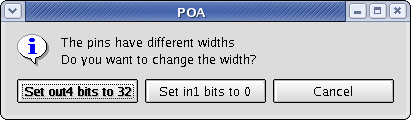
\includegraphics[width=10cm]{Pin}

\caption{POA Dialog}\label{test}

\end{center}

\end{figure}

\subsubsection{Verbindung automatisch routen}
Es gibt zwei verschiedene M"oglichkeiten des automatischen Routens:
\begin{itemize}
\item der Default Router ist der Standartrouter der automatisch beim erzeugen einer Verbindung benutzt wird.
\item der Smart Router kann nach Erzeugung einer Verbindung eingesetzt werden, um eventuell "uberlappende Verbindungen "uberlappungsfrei darzustellen.
\end{itemize}
Wenn man eine Verbindung automatisch routen m"ochte, w"ahlt man die Verbindung mit rechten Maustaste aus. Im Kontextmen"u den Eintrag {\bf Routen} w"ahlen und unter {\bf Routen} auf den gew"unschten Router ({\bf Default Router} oder {\bf Smart Router}) klicken.\newline
Der Smart Router kann auch durch ein Doppelklick auf die Verbindung gestartet werden.

\subsubsection{Verbindung manuell routen}
Zum manuellen Routen muss man die Verbindung mit der linken Maustaste ausw"ahlen. Nun kann man mit gedr"uckter Maustaste einen Verbindungsabschnitt entweder horizontal oder vertikal verschieben. Das hei"st ein horizontaler Verbindungsabschnitt kann nur vertikal verschoben werden und ein vertikaler Verbindungsabschnitt nur horizontal. Beim Verschieben der einzelnen Abschnitte werden die anh"angenden Linien automatisch nachgezogen, sodass eine Verbindung immer bestehen bleibt.

%%%%%%%%%%%%%%%%%%%%%%%%%%%%%%%%%%%%%%%%%%%%%%%%%%%%%%%%%%%%%%%%%%%%%%%%%%%%%
\subsection{Verbindung l"oschen}
Die zul"oschende Verbindung mit der rechten Maustaste ausw"ahlen. Im Kontextmen"u w"ahlt man nun den Eintrag {\bf Remove} und die Verbindung wird unwiderruflich gel"oscht.
Alternativ kann man die zul"oschende Verbindung mit der linken Maustaste ausw"ahlen und danach das Symbol {\bf L"oschen} in der Symbolleiste bzw. den Eintrag {\bf Remove} in der Men"uleiste anklicken oder die {\bf Entfernen} Taste auf der Tastatur dr"ucken.


%%%%%%%%%%%%%%%%%%%%%%%%%%%%%%%%%%%%%%%%%%%%%%%%%%%%%%%%%%%%%%%%%%%%%%%%%%%%%
%%%%%%%%%%%%%%%%%%%%%%%%%%%%%%%%%%%%%%%%%%%%%%%%%%%%%%%%%%%%%%%%%%%%%%%%%%%%%
\newpage
\section{Scheduling}
\begin{figure}[htbp]

\begin{center}

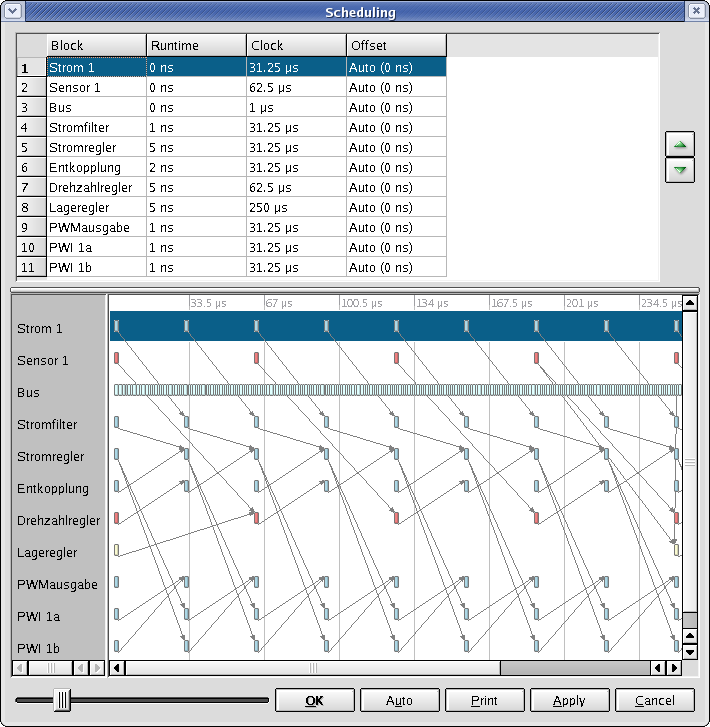
\includegraphics[width=15cm]{Scheduling1}

\caption{Scheduling}\label{test}

\end{center}
\end{figure}

Durch das Scheduling kann man eine Optimierung der Gesamtlaufzeit f"ur das CPLD-Board erreichen, indem man zum Beispiel die Offsetzeit der einzelnen Bl"ocke variiert oder Taktzeiten und Laufzeiten "andert, falls diese nicht schon festgelegt sind.\par
Den Scheduling Dialog kann man entweder "uber die Men"uleiste (Tools -> Scheduling) oder mit einem Kilck auf {\bf Scheduling} Symbol in der Symbolleiste "offnen.
Die aktuelle Konfiguration der Bl"ocke wird im Scheduling Dialog in der oberen Tabelle, in der alle Bl"ocke aufgelistet sind, angezeigt. Man hat die M"oglichkeit hier die Konfiguration (Laufzeit, Takt, Offset) der Bl"ocke zu "andern. Mit einem Doppelkick in die Zelle der Tabelle kann man nun entweder direkt "uber die Tastertur oder mit den Pfeiltasten in der Zelle die Ver"anderungen vornehmen.\par
Die Reihenfolge in der Tabelle bestimmt auch die Reihenfolge des Ablaufgraphen im unteren Teil des Dialogs. Aufgrund der "Ubersichtlichkeit des Ablaufgraphen ist es von Vorteil die Reihenfolge der Bl"ocke "andern zu k"onnen. Dazu muss man den Block mit der Maus markieren. Den markierten Block kann man nun mit den gr"unen Pfeiltasten nach oben oder unten verschieben, so dass im Ablaufgraph weniger "Uberkreuzungen der Kanten gibt. Mit dem Schieberegler am unteren linken Rand des Dialogs kann man die "Ubersichtlichkeit im Ablaufgraphen weiter verbessern. Indem man den Schieberegler nach rechts zieht und dadurch die Scalierung vergr"o"sert, wird der Ablaufgraph gestreckt und dadurch die Kanten besser zuordbar.\par

F"ur die manuelle Optimierung m"ussen die Offsets in der Tabelle per Hand eingegeben werden. Komfortabler geht die Optimierung, wenn man den {\bf Auto} Button dr"uckt. Dabei wird der {\bf Auto Scheduling} Dialog ge"offnet.
\begin{figure}[htbp]

\begin{center}

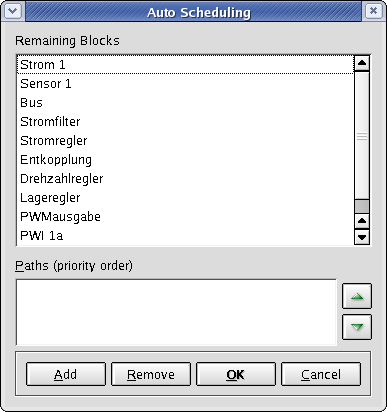
\includegraphics[width=8cm]{AutoScheduling}

\caption{Auto Scheduling}\label{test}

\end{center}
\end{figure}
Hier kann man priorisierte Pfade angeben, wonach die Optimierung abl"auft. Um einen priorisierten Pfad anzugeben oder hinzuzuf"ugen, klickt man auf den {\bf Add} Button. Dabei wird der Dialog {\bf Path Chooser} ge"offnet, indem man den Pfad angeben kann. Dazu muss man in der Auswahlbox {\bf Source Block} den Quellblock (z.B. ein Inputblock) und in der Auswahlbox {\bf Target Block} den Zielblock (z.B. ein Outputblock) angeben. Wenn man den Ausgangs- und Eingangspin der ausgew"ahlten Bl"ocke nicht angibt, werden alle M"oglichen Pfade zwischen den beiden Bl"ocken in einer Liste angezeigt, sonst nur die Pfade mit den entsprechenden Ausgangs- und Eingangspins.
\begin{figure}[htbp]

\begin{center}

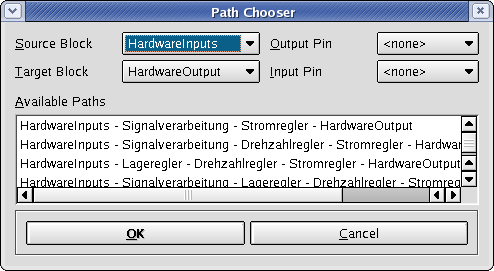
\includegraphics[width=8cm]{SchedulingPathChooser}

\caption{Path Chooser}\label{test}

\end{center}
\end{figure}
W"ahlt man nun aus der Liste einen priorisierten Pfad aus und best"atigt mit {\bf OK}, wird der Dialog geschlossen und man befindet sich wieder im {\bf Auto Scheduling} Dialog. Der ausgew"ahlte Pfad wird hier in die Priorit"atsliste hinzugef"ugt. Wenn man meherere priorisierte Pfade angegeben hat, kann man auch deren Reihenfolge (oben h"ochte Priorit"at) mit den gr"unen Pfeilen "andern. Mit der Best"adigung durch {\bf OK} wird die Optimierung in Abh"angigkeit der Priorit"aten durchf"uhrt.\newline
Wenn kein Pfad ausgew"ahlt und der {\bf OK} Button gedr"uckt wird, optimiert POA willk"urlich, d.h. ohne Priorit"aten.\newline
Mit {\bf Remove} kann man einen zuvor ausgew"ahlten Pfad aus der Priorit"atenliste l"oschen.

%%%%%%%%%%%%%%%%%%%%%%%%%%%%%%%%%%%%%%%%%%%%%%%%%%%%%%%%%%%%%%%%%%%%%%%%%%%%%
%%%%%%%%%%%%%%%%%%%%%%%%%%%%%%%%%%%%%%%%%%%%%%%%%%%%%%%%%%%%%%%%%%%%%%%%%%%%%
\newpage
\section{Deploy Project}
Mit {\bf Deploy Project} kann der Benutzer eine Plausibilit"atspr"ufung durchzuf"uhren, um eventuelle Fehler vor dem Downloadvorgang zu beseitigen. Bei der Pr"ufung des Projekt wird nach Inkonsistenz in den Bl"ocken und Verbindungen gesucht. Inkonsitenzen k"onnen sein , zum Beispiel: ID der CPU ist schon vergeben; verbundene Bl"ocke haben verschiedene Taktzeiten; Pins sind nicht verbunden; Verschiedene Bitbreiten bei einer Verbindung;... Wird ein Probleme bzw. Fehler entdeckt, so bekommt dieser einen Status (kritical, warning). Wenn keine Fehler entdeckt werden, wird der Status der Bl"ocke oder Verbindungen auf {\bf OK} gesetzt.\newline
Nach der Plausibilit"atspr"ufung kan man unter {\bf Deploy Project} den Programmcode der CPUs kompilieren und einzeln auf das CPLD-Board herunterladen.
\begin{figure}[htbp]

\begin{center}

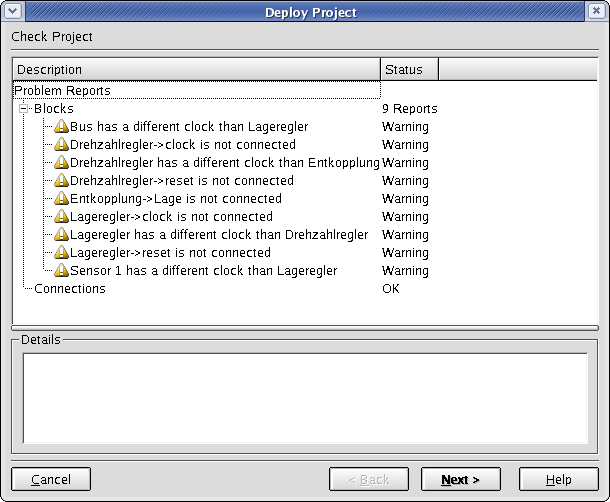
\includegraphics[width=10cm]{Deploy}

\caption{Deploy}\label{test}

\end{center}
\end{figure}
Um eine Plausibilit"atspr"ufung durchzuf"uhren, w"ahlt man im Men"u {\bf Tools} das Untermen"u {\bf Deploy Project}. Es wird der Dialog {\bf Deploy Project} ge"offnet, welcher die Befunde der Pr"ufung und deren Status kurz in einer Tabelle wiedergibt. Klickt man auf einen Eintrag in der Tabelle, so erscheint eine detailliertere Beschreibung des markierten Befunds.\par
Mit {\bf Cancel} kann man den Dialog verlassen und eventuelle Fehler korrigieren, um danach mit der Pr"ufung fortzufahren.\newline
Mit {\bf Next} kommt man in den n"achsten Dialog, in dem man den Programmcode der CPUs kompilieren und herunterladen kann. Dazu w"ahlt man in der Auswahlbox die CPU aus. Wenn man nun auf den Button {\bf Compile} dr"uckt, wird mit dem externe C-Compiler der zur CPU geh"orende Programmcode kompiliert. Dabei wird der {\bf POA Terminal} ge"offnet, um entsprechende Meldung auszugeben. Wird der {\bf Download} Button gedr"uckt, so wird das externe Download-Tool gestartet, um den kompilierten Code als {\bf Binary File} auf das CPLD-Board herunterzuladen.
Im {\bf Details} Bereich wird das Verzeichnis des Quellcodes und das der Bin"ardatei angegeben. Au"serdem kann man hier noch das Datum der letzten "Anderung unter {\bf Last Modified} ersehen.\par
\begin{figure}[htbp]

\begin{center}

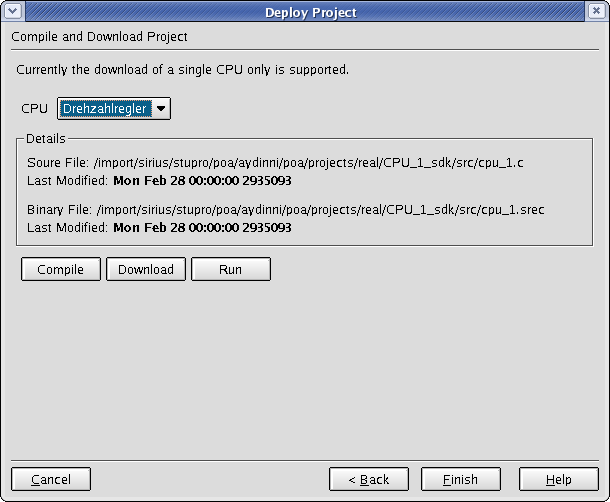
\includegraphics[width=10cm]{Deploy2}

\caption{Deploy}\label{test}

\end{center}
\end{figure}
Mit {\bf Back} kann man im Dialog zur"uck gehen, um eventuelle die Liste der Inkonsistenzen noch mal einzusehen.\par
Mit {\bf Finish} wird der {\bf Deploy Project} Dialog geschlossen und die "Anderungen gespeichert.

%%%%%%%%%%%%%%%%%%%%%%%%%%%%%%%%%%%%%%%%%%%%%%%%%%%%%%%%%%%%%%%%%%%%%%%%%%%%%
%%%%%%%%%%%%%%%%%%%%%%%%%%%%%%%%%%%%%%%%%%%%%%%%%%%%%%%%%%%%%%%%%%%%%%%%%%%%%%%
%% StuPro B, "Programmierumgebung Offener Antrieb" (POA)
%% Handbuch
%% $Id: definitionen.tex,v 1.3 2004/03/19 00:08:54 neco Exp $
%% Achtung: Diese Datei wird in das Handbuch inkludiert!
%%%%%%%%%%%%%%%%%%%%%%%%%%%%%%%%%%%%%%%%%%%%%%%%%%%%%%%%%%%%%%%%%%%%%%%%%%%%%%%
\newcommand{\begriff}[2]
{\item \bfseries{#1} \textnormal{#2}}

\chapter {Definitionen}
\begin{itemize}

\begriff{Ausgang}{Eine Speicheradresse auf die schreibend zugegriffen
  wird.}

\begriff{Block}{siehe Funktionsblock}

\begriff{Bus}{Mehrere Signalleitungen k"onnen zu einem Bus zusammen
  gefasst werden.}

\begriff{CPLD-Layout}{Anordnung von Funktionsbl"ocken und Signalleitungen.}

\begriff{CPLD}{Complex Programmable Logic Device}

\begriff{CPU}{Ein CPU-Block (auf Basis von NIOS).}

\begriff{Core}{Eine festgelegte Logik mit bekannter Laufzeit.}

\begriff{Download}{Herunterladen eines vollst"andig kompilierten CPLD-Layouts
auf das CPLD.}

\begriff{Eingang}{Eine Speicheradresse auf die lesend zugegriffen wird.}

\begriff{Episodisches Signal}{Ein Eingang oder Ausgang.}

\begriff{Funktionsblock}{Virtuelles Abbild eines Cores, einer CPU oder
eines Ein- bzw. Ausgabeblocks.}

\begriff{ISWOS}{Minimal-Betriebssystem, dass nach der Initialisierung
  des CPLDs auf den CPUs ausgef"uhrt wird.}

\begriff{Laufzeitermittlung}{Absch"atzung der maximalen Laufzeit eines
  Programms in Milli-Sekunden.}

\begriff{Offset}{Anzahl Takte bevor ein Funktionsblock zum ersten Mal
  angestossen wird.}

\begriff{Optimierung}{Verk"urzung der Gesamtlaufzeit eines CPLD-Zyklus.}

\begriff{Periode}{Anzahl Takte nach denen ein Funktionsblock erneut
  gestartet wird}

\begriff{Plausibilit"aspr"ufung}{Pr"ufung des CPLD-Layouts auf
  unverkn"upfte und falsch verkn"upfte Eingangs/Ausgangspins.}

\begriff{Scheduler}{Hardware, die Funktionsbl"ocke periodisch startet}

\begriff{Signalleitung}{Eine Verbindung zwischen zwei
  Funktionsbl"ocken. Eine Signalleitung hat immer 32-bit.}

\begriff{Takt}{Kleinste Zeiteinheit des Schedulers}

\begriff{Verbindung}{Eine Kopplung von einem Ausgang zu ein oder
  mehreren Eing"angen.}

\end{itemize}


\end{document}
